\chapter{Graphic Design}\label{graphic-design}
During the specification phase I prioritized the features and planned how many pages are needed and what kind of components are needed to provide the features for the user \see{design-specification}. Then I drew some sketches to see how these components would look like altogether \see{appendix-design-sketches}. The next step was to decide what kind of design elements and templates I want to use to create the planned layouts.

\section{Design template}

To show only a specific set of information I have decided to use a minimalist design. A minimalist design is a clear design, focusing on typography, space, color and basic design elements. This way the portal will show as much information as the user needs with as few elements as possible. 

To look for templates and ideas I read the Designmodo blog~\cite{Designmodo} and checked all the popular websites, e.g., Facebook, Github, Twitter and Medium. Designmodo also have purchasable website builders, like Slides~\cite{Designmodo-slides}, but I prefer the simple design of the Bootstrap elements~\cite{Bootstrap}. 

Bootstrap is a free and open source HTML, CSS and JS framework to create responsive design. It was originally a part of Twitter as Twitter Blueprint, but in 2011 it was released as an open source project. Bootstrap contains elements for responsive web design and mobile design. Bootstrap 4 alpha was launched in August 2015 alongside with a new side project, Official Bootstrap Themes~\cite{Bootstrap-themes}. Bootstrap Themes are purchasable redesigned collections of Bootstrap components with new components and plug-ins. Although I really like these themes, I will use the free components, because it does not worth buying any theme if I will change some parts of the included components. 

\subsection{Colors}

After deciding what kind of design framework will I use, I had to choose the colors of the portal. Both the Budapest University of Technology and Economics~\cite{BME-Arculat}~\cite{BME-Arculat-Intranet} and the Faculty of Electrical Engineering and Informatics~\cite{VIK-Arculat}~\cite{VIK-Arculat-PDF} have their own Visual Identity Guidelines. A visual identity guideline contains the description of which color is the official color of the institution and in what kind of text which fonts and why that specific font should be used.

I consulted with my advisor, Sándor Gajdos and he advised me that I should not follow any of these visual identity guidelines. Following any of the strict guidelines can be a problem in the future, if someone would like to use this portal for another course that does not belong to the faculty or the university. Based on my subjective opinion I have decided to use green as the main color of the portal. I used the Google Color palette~\cite{google-color-chart} to choose a nice green, changed it a bit, and I got the final color, \#2a623d.

\newpage
\section{New Graphic Design}

Beside the newer, modern design, I wanted to make sure that the users of the old portal can easily do the same tasks in the new portal too. The pages are separated by features and the different states of the laboratory page will be separated with tabs.

\begin{figure}[!ht]
	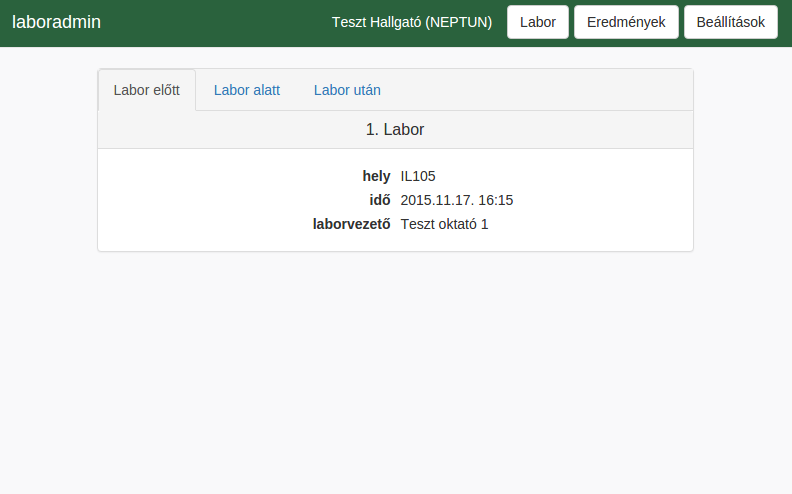
\includegraphics[width=\textwidth]{figures/design/labor_elott.png}
	\caption{Before laboratory}
	\label{fig:before}
\end{figure}

%\begin{figure}[!ht]
%	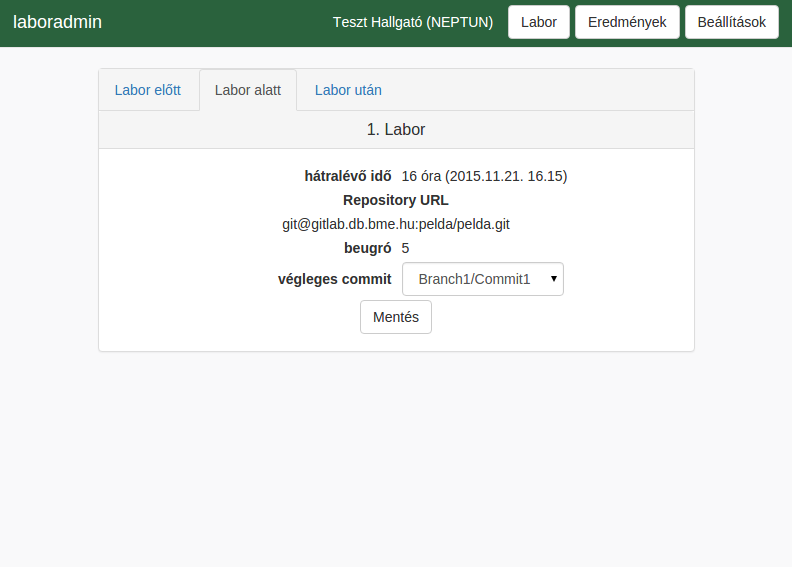
\includegraphics[width=\textwidth]{figures/design/labor_alatt.png}
%	\caption{During laboratory}
%	\label{fig:during}
%\end{figure}



\begin{figure}[!ht]
	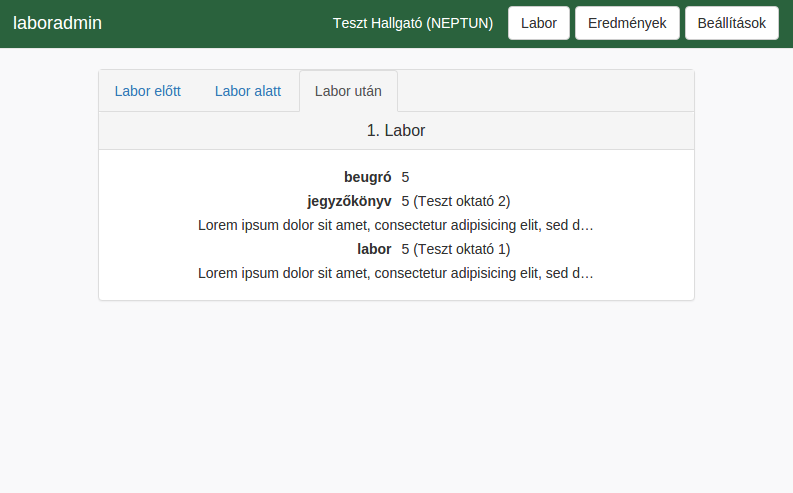
\includegraphics[width=\textwidth]{figures/design/labor_utan.png}
	\caption{After laboratory}
	\label{fig:after}
\end{figure}

\begin{figure}[!ht]
	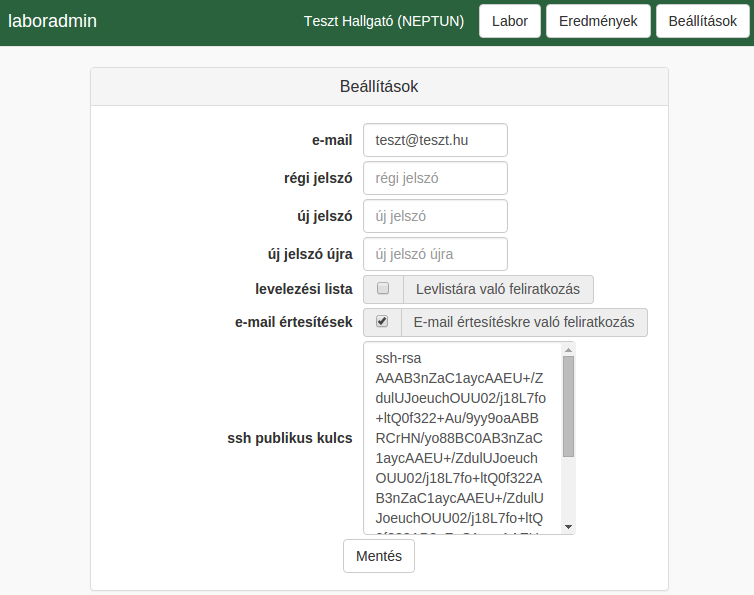
\includegraphics[width=\textwidth]{figures/design/beallitasok.png}
	\caption{Settings}
	\label{fig:settings}
\end{figure}

\begin{figure}[!ht]
	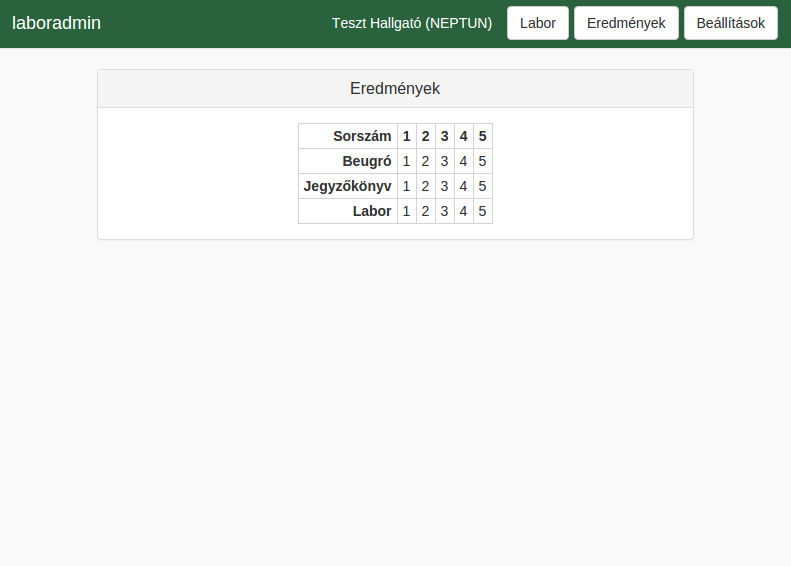
\includegraphics[width=\textwidth]{figures/design/eredmenyek.png}
	\caption{Summarized results}
	\label{fig:results}
\end{figure}

\begin{figure}[!ht]
	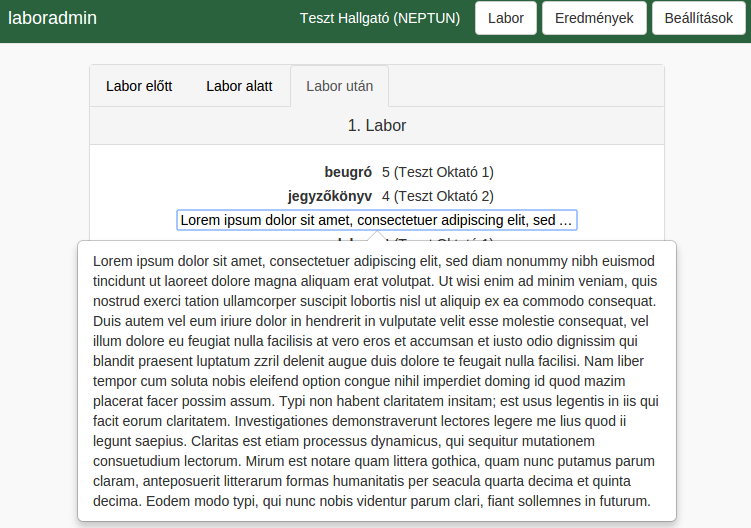
\includegraphics[width=\textwidth]{figures/design/popup.png}
	\caption{Popover for reviews.}
	\label{fig:popup}
\end{figure}

